% Options for packages loaded elsewhere
\PassOptionsToPackage{unicode}{hyperref}
\PassOptionsToPackage{hyphens}{url}
\documentclass[
]{book}
\usepackage{xcolor}
\usepackage{amsmath,amssymb}
\setcounter{secnumdepth}{5}
\usepackage{iftex}
\ifPDFTeX
  \usepackage[T1]{fontenc}
  \usepackage[utf8]{inputenc}
  \usepackage{textcomp} % provide euro and other symbols
\else % if luatex or xetex
  \usepackage{unicode-math} % this also loads fontspec
  \defaultfontfeatures{Scale=MatchLowercase}
  \defaultfontfeatures[\rmfamily]{Ligatures=TeX,Scale=1}
\fi
\usepackage{lmodern}
\ifPDFTeX\else
  % xetex/luatex font selection
\fi
% Use upquote if available, for straight quotes in verbatim environments
\IfFileExists{upquote.sty}{\usepackage{upquote}}{}
\IfFileExists{microtype.sty}{% use microtype if available
  \usepackage[]{microtype}
  \UseMicrotypeSet[protrusion]{basicmath} % disable protrusion for tt fonts
}{}
\makeatletter
\@ifundefined{KOMAClassName}{% if non-KOMA class
  \IfFileExists{parskip.sty}{%
    \usepackage{parskip}
  }{% else
    \setlength{\parindent}{0pt}
    \setlength{\parskip}{6pt plus 2pt minus 1pt}}
}{% if KOMA class
  \KOMAoptions{parskip=half}}
\makeatother
\usepackage{graphicx}
\makeatletter
\newsavebox\pandoc@box
\newcommand*\pandocbounded[1]{% scales image to fit in text height/width
  \sbox\pandoc@box{#1}%
  \Gscale@div\@tempa{\textheight}{\dimexpr\ht\pandoc@box+\dp\pandoc@box\relax}%
  \Gscale@div\@tempb{\linewidth}{\wd\pandoc@box}%
  \ifdim\@tempb\p@<\@tempa\p@\let\@tempa\@tempb\fi% select the smaller of both
  \ifdim\@tempa\p@<\p@\scalebox{\@tempa}{\usebox\pandoc@box}%
  \else\usebox{\pandoc@box}%
  \fi%
}
% Set default figure placement to htbp
\def\fps@figure{htbp}
\makeatother
\ifLuaTeX
\usepackage[bidi=basic]{babel}
\else
\usepackage[bidi=default]{babel}
\fi
\babelprovide[main,import]{italian}
% get rid of language-specific shorthands (see #6817):
\let\LanguageShortHands\languageshorthands
\def\languageshorthands#1{}
\setlength{\emergencystretch}{3em} % prevent overfull lines
\providecommand{\tightlist}{%
  \setlength{\itemsep}{0pt}\setlength{\parskip}{0pt}}
          \usepackage{cancel}
          \usepackage[backend=biber]{biblatex}
          \bibliography{citazioni}
          \addbibresource{citazioni.bib}
          \usepackage{comment}
          \usepackage{float}
          \usepackage{multirow}
          \usepackage{subcaption}
          \usepackage{svg}
          \usepackage{tikz}
          \usetikzlibrary{patterns}
          \usepackage[version=4]{mhchem}
          \usepackage{circuitikz}
          \usepackage{pgfplots}
          \usepackage{steinmetz}
          \usepackage{derivative}
          \usepackage{tabularray}
          \usepackage{mathtools}
          \usepackage{siunitx}
          \usepackage{tcolorbox}
          \usepackage{geometry}
          \usepackage{array}
          \usepackage{caption}
          \usepackage{sectsty}
          \usepackage{hhline}
              \geometry{
                  a4paper,
                  total={170mm,257mm},
                  left=20mm,
                  top=20mm,
              }
          \tcbuselibrary{most}
          \newtcolorbox[auto counter,number within=section]{mybox}[1]{colback=red!5!white, colframe=red!75!black,
          fonttitle=\bfseries, title={#1}}
          \newtcolorbox[auto counter,number within=section]{mybox2}[1]{colback=green!5!white, colframe=green!75!black,
          fonttitle=\bfseries, title={#1}}
          \newtcolorbox[auto counter,number within=section]{bluebox}[1]{colback=blue!5!white, colframe=blue!75!black,
          fonttitle=\bfseries, title={#1}}
\usepackage{bookmark}
\IfFileExists{xurl.sty}{\usepackage{xurl}}{} % add URL line breaks if available
\urlstyle{same}
\hypersetup{
  pdftitle={Appunti Elettronica Digitale},
  pdfauthor={Leonardo Toccafondi},
  pdflang={it},
  pdfsubject={Elettronica},
  hidelinks,
  pdfcreator={LaTeX via pandoc}}

\title{Appunti Elettronica Digitale}
\author{Leonardo Toccafondi}
\date{2024-04-12}

\begin{document}
\frontmatter
\maketitle

{
\setcounter{tocdepth}{2}
\tableofcontents
}
\mainmatter
\chapter{Dispositivi elettronici}\label{dispositivi-elettronici}

\section{Semiconduttori}\label{semiconduttori}

I semiconduttori sono i materiali con cui sono composti i circuiti
integrati. Sono, come suggerisce il nome, materiali in cui il flusso di
corrente \emph{non è libero} (non è un conduttore), ma è
\textbf{presente} (non è un'isolante).

In particolare, conducono in particolari situazioni. Quali sono però i
materiali con queste condizioni?

\begin{itemize}
\tightlist
\item
  \emph{Elementi semiconduttori}: Silicio (\ce{Si}), Germanio (\ce{Ge})
  (Carbonio (\ce{C}), ma composto)
\item
  \emph{Elementi composti}: \ce{GaAs}, \ce{GaN} (Gallio-Arsenico/Azoto)
  In generale sono gli elementi della \(14°\) colonna della tavola
  periodica o composti a numero medio di elettroni liberi pari a 4 (dai
  3 ai 4).
\end{itemize}

\begin{mybox}{\emph{Silicio}}
Il silicio è il materiale semiconduttore sicuramente più diffuso. \newline
Un atomo presenta 4 elettroni (detti di \emph{valenza}) nello strato più esterno,
ma sua forma cristallina pura del silicio ogni atomo forma un legame covalente
\footnote{legame chimico in cui due atomi mettono in comune delle coppie di elettroni.}
con i suoi vicini "più prossimi".
Il cristallo di silicio puro ha inoltre una struttura cristallina matriciale,
che blocca il passaggio di carica. \newline
È da notare che all'aumentare della temperatura, qualche elettrone può rompere il legame
e muoversi liberamente nel cristallo.
\end{mybox}

Per dotare un materiale semiconduttore di conduttività \emph{selettiva}
è necessario \emph{``drogare''} il materiale stesso. Il drogaggio,
quindi, va a \textbf{modificare} la concentrazione di elettroni e di
\emph{lacune} \footnote{Assenza di elettroni dovuta alla
  \textbf{rottura} di un legame. È insieme all'elettrone, un portatore
  di carica nei semiconduttori.}, attraverso questo inserimento di
impurità sostituzionali (ovvero atomi di elementi diversi, i quali si
sostituiscono ad alcuni degli atomi di silicio.) \newline In pratica
andiamo ad aggiungere, in piccole dosi, nel reticolo cristallino
materiali della \(5°\) colonna (drogaggio di tipo \textbf{n}, hanno 5
elettroni di valenza, sono detti \textbf{donatori}, ad esempio il
fosforo), o elementi della \(3°\) colonna (tipo \textbf{p}, hanno 3
elettroni di valenza e sono detti \textbf{accettori}, ad esempio il
boro).\newline Tale discrepanza induce la formazione di livelli
energetici aggiuntivi all'interno della banda proibita\footnote{Intervallo
  di energia interdetto agli elettroni, distanza tra la banda di valenza
  di conduzione (nei semiconduttori distanti \(1\si{eV}\)).} o ``gap''
del semiconduttore. Nel primo caso si genera un eccesso di lacune, le
quali si comportano come particelle cariche \emph{positivamente}, mentre
nel secondo si ha un eccesso di elettroni liberi, determinando così una
variazione della conducibilità elettrica intrinseca del materiale.
\newline Non solo, sia le lacune che gli elettroni liberi sono quindi
liberi di muoversi all'interno del semiconduttore!

La qualità del semiconduttore è influenzata dal materiale usato (per
esempio Ge è meglio del \ce{Si}, ma è più raro), che è a sua volta
influenzato dal goal\footnote{(penso voglia dire ``obiettivo
  perseguito'').} (elettronica digitale usa \ce{Si}, l'elettronica di
potenza il \ce{GaN} o \ce{SiC}).

Vediamo ora degli elementi in silicio.

\subsection{Giunzione p-n}\label{giunzione-p-n}

Una giunzione pn (o p-n) si forma quando una del materiale
semiconduttore intrinseco \footnote{Puro, quindi privo di un
  quantitativo significativo di drogaggio.} drogato con un drogaggio p
(con una percentuale \(N_{A}\), n.~accettori) viene posta a contatto con
altro materiale semiconduttore drogato con un drogaggio n (con una
percentuale \(N_{D}\), n.~donatori). \newline La concentrazione di ioni
dalle seguenti ``formule'': \[
N_A = \frac{\# acceptors}{vol. unit} \text{ e } N_D=\frac{\# donors}{vol. unit}
\] dove \(N_a\) indica il numero\footnote{Oppure densità di ioni, o
  concentrazione\ldots{}} di ioni di tipo p:`positivo', mentre \(N_d\)
il numero di ioni di tipo n:`negativo'.

Collegando un blocco drogato tipo p ed uno tipo n abbiamo
(idealmente)\footnote{Nella pratica parto da un blocco puro di silicio,
  per poi iniettare a \emph{strati} il drogaggio.}

\begin{figure}[H]
\centering
\begin{tikzpicture}[scale=1.75]
    \draw[very thick](-2,0)--(2,0)--(2,1)--(-2,1)--(-2,0);
    \draw[very thick](0,0)--(0,1);
    \draw[thick](0.5,0)--(0.5,1);
    \draw[thick](-0.5,0)--(-0.5,1);
    \node at (1.25,0.5) {$N$};
    \node at (-1.25,0.5) {$P$};
     % Aggiungiamo le due righe orizzontali
    \draw[thick](-2.5,0.5)--(-2,0.5);
    \draw[thick](2,0.5)--(2.5,0.5);
    \draw[->](-0.25,0.5)--(0.25,0.5)node[above]{$V_0$};
\end{tikzpicture}
\caption{Giunzione pn}
\end{figure}

Il materiale quindi è separato in due zone \emph{nettamente distinte},
senza alterazione della struttura cristallina all'interfaccia delle due
zone. \newline L'abbondanza di lacune in p è, come sappiamo,
corrispondente ad una carenza di elettroni, di cui n \emph{abbonda}. In
altre parole questa diversa \emph{densità} di portatori di carica genera
una \textbf{migrazione} di elettroni da N verso P, detta anche
\emph{diffusione\footnote{Fenomeno che si ritrova in natura qualora vi
  sia uno squilibrio nella distribuzione nello spazio di particelle
  simili.} (elettrica)} \(I_D\) oppure anche \emph{corrente di
diffusione}, che consiste quindi in

\begin{itemize}
\tightlist
\item
  lacune che si diffondono dalla regione (dal semiconduttore) drogata
  con p alla regione n;
\item
  elettroni che si diffondono dalla regione drogata con n alla regione
  p.
\end{itemize}

\begin{quote}
N.B.: Nella zona n i \textbf{portatori maggioritari} di carica sono le
cariche negative, mentre nella zona p sono le cariche positive
\end{quote}

Tale fenomeno carica in modo \emph{positivo} il semiconduttore drogato n
(meno elettroni), e in modo \emph{negativo} il semiconduttore drogato p
(più elettroni). \newline Le lacune che si diffondono dalla regione/zona
p alla n si ricombinano con gli elettroni liberi, \emph{scomparendo}. Di
conseguenza, il numero di elettroni liberi nella zona n
\emph{diminuisce}, quindi non saranno più neutralizzate alcune cariche
fisse positive (atomi donatori). Dal momento che questa ricombinazione
avviene in prossimità della giunzione, accanto a questa si svilupperà
una regione \textbf{svuotata} di elettroni, con cariche fisse positive
non compensate. \newline Analogamente nella zona p otterremo una zona
svuotata dalle lacune e che comprende delle cariche fisse (in questo
caso negative) non compensate. \newline Entrambe queste zone danno luogo
alla \textbf{regione di svuotamento}\footnote{Svuotata di portatori
  \textbf{mobili}} (o di carica spaziale, in inglese \emph{depletion
layer}). Inoltre lo spostamento delle cariche crea a cavallo della
giunzione un campo elettrico, con la zona n positiva rispetto alla zona
p.~La presenza del campo elettrico comporta la presenza di una
differenza di potenziale. Questa è anche detta \textbf{barriera di
potenziale}\footnote{È possibile superarla, ma deve essere fornita una
  differenza di potenziale \textbf{esterna}.}, in quanto si oppone ad
un'ulterore diffusione ai portatori di carica soggetti alla spinta della
diffusione (si oppone al movimento di elettroni nella regione p e lacune
nella regione n). Una volta che la corrente di diffusione equivale la
corrente di trascinamento\footnote{Detta anche corrente di deriva
  (drift), in questo caso i portatori si muovono perché \textbf{spinti}
  dal campo elettrico dovuto allo squilibrio di carica.} \(I_S\)
raggiungiamo un \textbf{equilibrio} (dinamico): La presenza del campo
elettrico comporta la presenza di una differenza di potenziale.

\begin{figure}[H]
\centering
\begin{subfigure}[t]{0.6\textwidth}
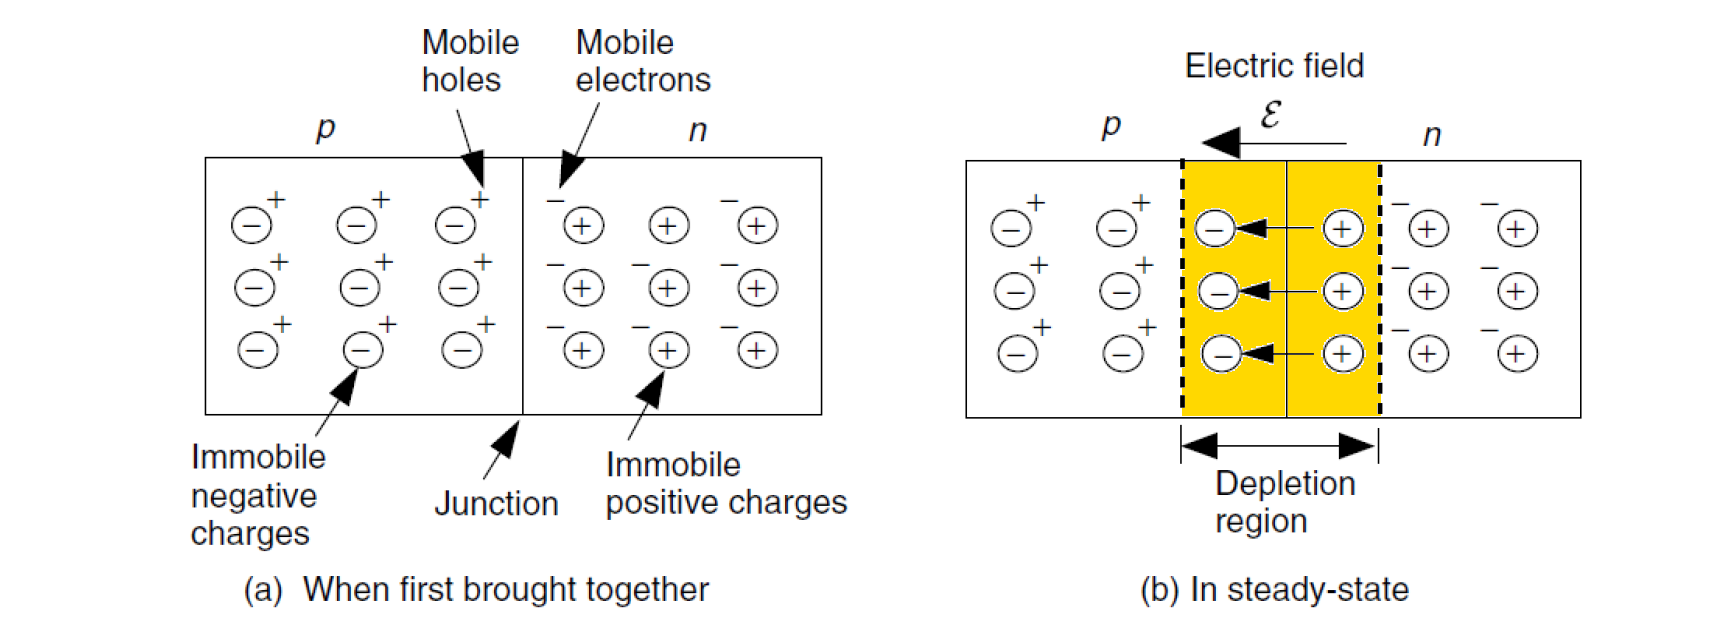
\includegraphics[width=\textwidth,height=\textheight,keepaspectratio]{immagini/1.png}
\caption{Regione di svuotamento}
\end{subfigure}
\begin{subfigure}[t]{0.3\textwidth}
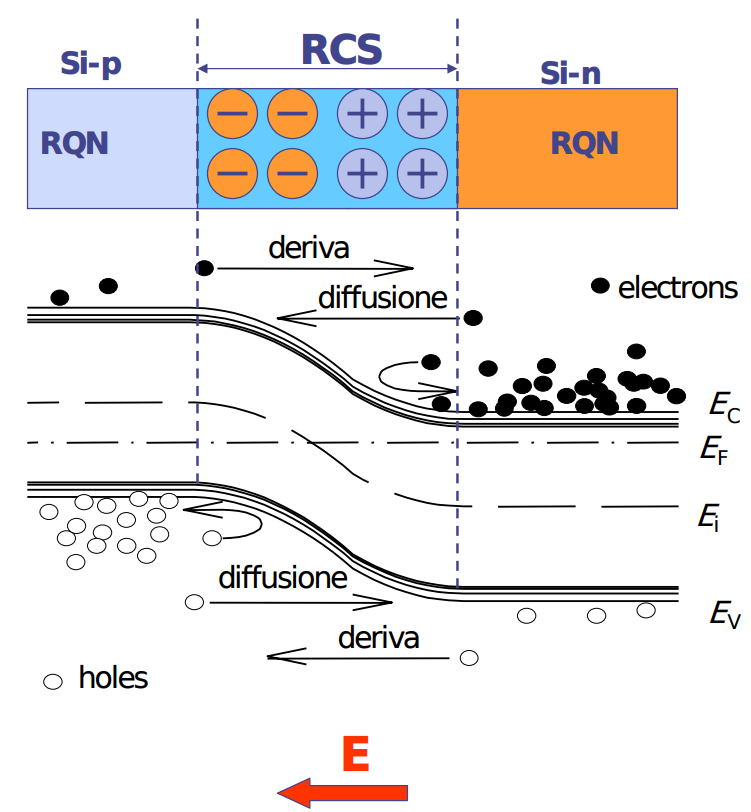
\includegraphics[width=\textwidth,height=\textheight,keepaspectratio]{immagini/pn_equilibrio.png}
\caption{Giunzione pn all'equilibrio}
\end{subfigure}
\end{figure}

In genere la regione di svuotamento non è simmetrica: la seguente
equazione regola la larghezza della regione: \[
x_p N_A = x_N N_D
\] dove \(x_p\) e \(x_n\) sono rispettivamente le \textbf{larghezze}
della regione di svuotamento entro il semiconduttore drogato p e drogato
n.

\begin{figure}[H]
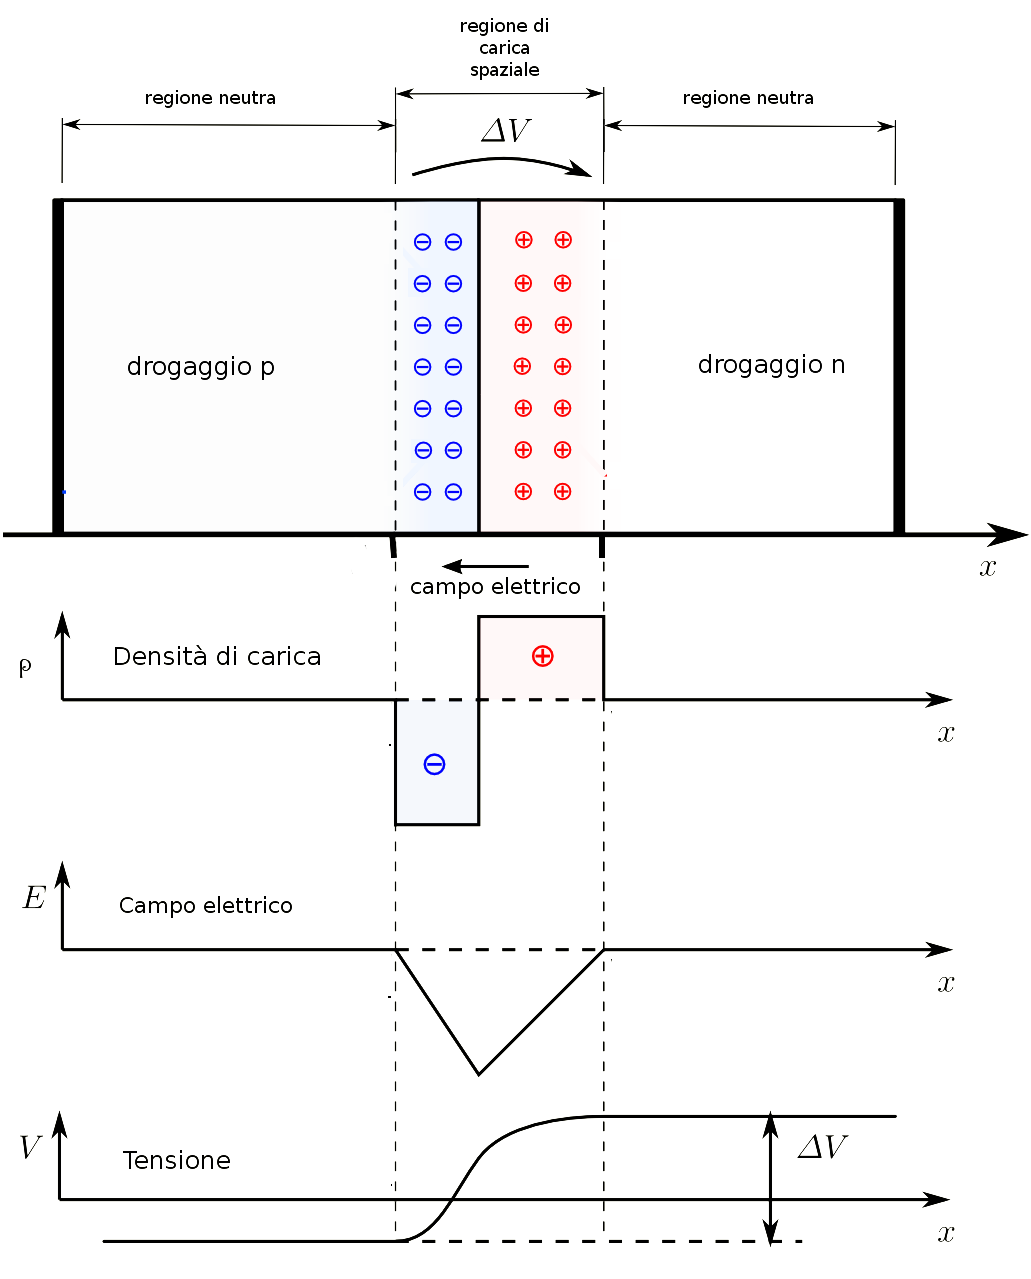
\includegraphics[height=0.6\textwidth, width=!]{immagini/2.png}
\centering
\caption{Grafici relativi al potenziale, al campo elettrico e alla carica nella giunzione pn}
\label{fig:1.3}
\end{figure}

Come si vede nella @fig:1.3 :

\begin{itemize}
\tightlist
\item
  \(N_A > N_D \to\) più è drogata la regione più la regione di
  svuotamento è piccola.
\end{itemize}

\section{I diodi}\label{i-diodi}

Il simbolo circuitale della giunzione p-n, detta
\textbf{diodo}\footnote{Il diodo ideale è un dispositivo che lascia
  passare corrente solo in un senso, con resistenza nulla, e non lascia
  passare corrente nell'altro senso. Il diodo a giunzione approssima
  molto bene un diodo ideale, ed è l'elemento circuitale non lineare più
  importante.} è

\begin{figure}[h]
\begin{centering}
\begin{circuitikz}
  \draw (0,0) node[left]{A} to[diode,color=red] (2,0) node[right]{K};
\end{circuitikz}
\caption{Diodo}
\end{centering}
\end{figure}

dove a sinistra abbiamo un \textbf{anodo} A (dal greco \emph{salita}), e
a destra un \textbf{catodo} K (dal greco \emph{discesa}).

Sia la zone p che la zona n sono munite di un contatto elettrico (detto
\textbf{reoforo}), in modo tale che sia possibile applicarvi una
tensione.

\subsection{Polarizzazione}\label{polarizzazione}

L'applicazione di un potenziale sul diodo viene detta
\textbf{polarizzazione}, e si distingue la:

\begin{itemize}
\tightlist
\item
  Polarizzazione \textbf{diretta} (forward bias): applico un potenziale
  positivo sull'anodo A (lato p) e negativo sul catodo K (lato n). La
  differenza di potenziale applicata ha la polarità \emph{concorde} con
  la barriera di potenziale.

  \begin{itemize}
  \tightlist
  \item
    L'aumento della tensione determina una riduzione della barriera di
    potenziale, e di conseguenza della larghezza della regione di
    svuotamento. In questo modo aumenta il numero di elettroni e di
    lacune capaci di attraversare la giunzione tramite la diffusione.
  \item
    La corrente di diffusione, rispetto a quella di deriva, aumenta
    rapidamente di svariati ordini di grandezza.

    \begin{figure}[h]
    \begin{centering}
    \begin{circuitikz}
    \draw (0,0) node[left]{+} to[diode,color=blue] (2,0) node[right]{-};
    \end{circuitikz}
    \caption{Diodo polarizzato direttamente}
    \end{centering}
    \end{figure}
  \end{itemize}
\item
  Polarizzazione \textbf{indiretta} (reverse bias): applico un
  potenziale negativo sull'anodo e positivo sul catodo. In questo caso
  la polarità della tensione applicata è discorde rispetto a quella
  della barriera di potenziale.

  \begin{itemize}
  \tightlist
  \item
    La regione di svuotamento si allarga, e la tensione di
    polarizzazione richiama le lacune verso il terminale negativo e gli
    elettroni verso il terminale positivo. Quindi l'ampiezza della
    barriera di potenziale aumenta.
  \item
    La corrente di diffusione diminuisce fino ad annullarsi, mentre
    quella di deriva rimane (anche se è molto piccola e varia con la
    temperatura). Quindi quasi nessuna corrente riesce a scorrere.
  \item
    Il campo elettrico incrementa fino ad ottenere il \emph{breakdown}.
  \end{itemize}
\end{itemize}

\begin{figure}[h]
\begin{centering}
\begin{circuitikz}
  \draw[thick] (0,0) node[left]{-} to[diode,color=orange] (2,0) node[right]{+};
\end{circuitikz}
\caption{Diodo polarizzato indirettamente}
\end{centering}
\end{figure}

\subsection{Equazione caratteristica e
breakdown}\label{equazione-caratteristica-e-breakdown}

In generale, la giunzione pn ha un'equazione caratteristica

\[
i=I_{S}(e^{\frac{V_d}{nV_t}}-1)
\]

detta \textbf{equazione di Shockley}:

\begin{itemize}
\tightlist
\item
  \(V_d\) indica la differenza di potenziale applicati ai capi del
  diodo;
\item
  \(nV_t\) è il potenziale nativo dei diodi (pari a
  \(\SI{0.7}{\volt}\)), o \emph{tensione termica}, pari a
  \(\SI{26}{\mV}\).
\item
  \(I_S\) (o \(I_0\)) è una costante detta \emph{corrente di
  saturazione} (per il \ce{Si} ha valori tra \(10^{-15}\) e
  \(10^{-19} \, \si{\ampere}\))
\end{itemize}

In condizioni di polarizzazione diretta la corrente è trascurabile per
tensioni al di sotto di \(0,5 - 0,6 \si{\volt}\) (per diodi al silicio)
e dopo aver superato la \emph{tensione di soglia} cresce molto
repentinamente\footnote{Per un aumento di corrente di un fattore mille è
  sufficiente un aumento di tensione pari a \(\SI{0.8}{\volt}\). Infatti
  viene assunta \(\SI{0.6}{\volt}\) come tensione di soglia e
  \(\SI{0.8}{\volt}\) come tensione massima.}. \newline Quando il diodo
è in polarizzazione inversa, aumentando la tensione la corrente rimane
costante finché non si raggiunge la cosiddetta \textbf{tensione di
breakdown} (o di rottura). Una volta oltrepassata la corrente aumenta
\colorbox{yellow}{(forse in questo caso \textit{diminuisce})} in maniera
drastica a tensione praticamente costante.

\begin{mybox2}{Il \emph{breakdown}}
Il fenomeno del breakdown è dovuto a:
\begin{enumerate}
\item Effetto \emph{Zener}: prevalente per tensioni di breakdown inferiori alla decina di volt. Quando il diodo è polarizzato
    inversamente e la tensione è compresa tra $0\si{\volt}$ e $V_Z$ (inferiore a zero), si comporta quasi come un circuito aperto,
    seppur continui a scorrere una piccola corrente di saturazione inversa, oltre $V_Z$ la banda di valenza della regione p si
    avvicina talmente tanto alla banda di conduzione che alcuni elettroni si spostano dall'una all'altra;
\item Effetto \emph{valanga} (avalanche): prevalente per tensioni di breakdown superiori alla decina di volt. Si manifesta
    in presenza di campi elettrici \emph{molto elevati}, dovuti alla presenza di una tensione "moderata", ma imposta su distanze
    molto corte.
\end{enumerate}

Solitamente il processo del breakdown è irreversibile, tranne per i diodi Zener, i quali sono ideati per andare in breakdown.
\end{mybox2}

\begin{figure}[H]
    \centering
    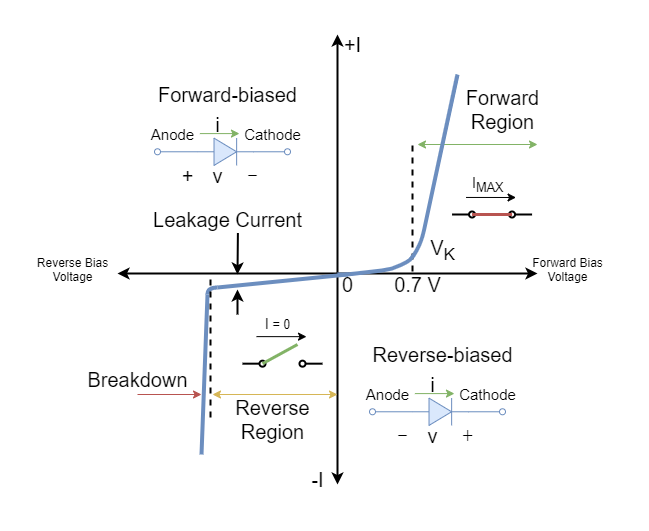
\includegraphics[width=0.7\textwidth]{immagini/iv_pn.png} % replace with your image file
    \caption{Una tipica caratteristica I-V di un diodo a giunzione PN \autocite{diodeMS}}
    \label{fig:caratteristica_pn}
\end{figure}

\subsection{Diodi Speciali}\label{diodi-speciali}

\subsubsection{Fotodiodi}\label{fotodiodi}

I fotodiodi sono diodi in cui la giunzione è ``scoperta'', o incapsulata
in un materiale trasparente, in quanto vogliamo che sia in grado di
\textbf{emettere} una corrente elettrica sfruttando l'effetto
fotoelettrico. Difatti è un \emph{trasduttore}\footnote{Dispositivo in
  grado di convertire una forma di energia in una diversa.} da un
segnale ottico ad un elettrico. \newline L'equazione caratteristica del
fotodiodo è pari a quella di un diodo normale, con l'aggiunta di un
termine \(I_{ph}\), che rappresenta la corrente
\emph{fotogenerata}\footnote{Risulta proporzionale al flusso di fotoni
  che colpiscono il fotodiodo}: \[
i=I_{S}(e^{\frac{V_d}{nV_t}}-1)-I_{ph}
\]

\begin{center}
\begin{circuitikz}
  \draw (0,0) node[left]{+} to[diode, l_=Diodo normale] (2,0) node[right]{-};
  \draw[pD={}, l_=Fotodiodo] (4,0) node[left]{+} to node[right]{-} (6,0);
\end{circuitikz}
\end{center}

I fotodiodi p-n possono essere utilizzati senza essere polarizzati: sono
adatti per ``applicazioni'' in situazioni di bassa luminosità. Quando
sono illuminati, il campo elettrico nella regione di deplezione aumenta,
producendo la corrente fotogenerata la quale è cresce all'aumentare del
flusso di fotoni. \newline Altrimenti i fotodiodi operano in
\emph{polarizzazione inversa}, in modo tale che i fotoni (del colore
``giusto'') possedano energia sufficiente ad oltrepassare la barriera di
potenziale e a condurre quindi corrente elettrica.

\subsubsection{Led}\label{led}

I \textbf{led} (\emph{light emitting diode}) è un tipo di diodo che
\textbf{converte} energia elettrica in luce. Sono formati da sottili
strati di materiali semiconduttori fortemente drogati, i quali
caratterizzano i diversi colori emessi quando viene applicata una
polarizzazione \emph{diretta}.\newline Da un punto di vista
\emph{costruttivo} i led sono ricoperti da uno strato spesso di
resina\footnote{Epossidica, in inglese \emph{epoxy}.}
\textbf{trasparente} di forma emisferica, sia per proteggere il led
stesso sia per convogliare la luce emessa.

\begin{figure}[h]
\centering
\begin{circuitikz}[american]
\draw[pD={}](0.5,-0.5)to(2.0,-0.5);
\end{circuitikz}
\caption{Simbolo circuitale di un led}
\end{figure}

Applicando quindi una tensione positiva all'anodo, riduciamo la barriera
di potenziale, in modo tale che elettroni e lacune ricombinandosi
generino fotoni pari al gap tra la banda di conduzione e quella di
valenza.

Come si può vedere nella tabella sottostante, al fine di generare un
colore visibile, deve essere fornita una tensione almeno pari a
\(1,5 \si{\volt}\)

\begin{table}[H]
    \centering
    \begin{tabular}{|c|c|c|c|}
    \hline
        \textbf{Semiconduttore composto} & \textbf{$V_{F}$ a $20$ mA} & \textbf{Banda di lunghezza d'onda} & \textbf{Colore} \\ \hline
        GaInN & 4.0V & 450 nm & Bianco \\ \hline
        SiC & 3.6V & 430-505 nm & Blu \\ \hline
        GaAsP & 22V & 585-595 mm & Giallo \\ \hline
        GaAsP & 2.0V & 605-620nm & Ambra \\ \hline
        GaAsP & 1.8V & 630-660nm & Rosso \\ \hline
        GaAs & 1.2V & 850-940nm & Infrarosso \\ \hline
    \end{tabular}
    \caption{Diverse tipologie di led in base al colore prodotto}
\end{table}

\subsubsection{Diodo Schottky}\label{diodo-schottky}

In questa tipologia di diodo la giunzione p-n è data dall'unione del
metallo (che svolge il ruolo della regione p) con un materiale
semiconduttore drogato n.~In questo modo si viene a creare una
\emph{``barriera Schottky''}: questa, a differenza della giunzione p-n
standard, ha una \emph{bassa} tensione di giunzione (o tensione di
soglia). Infatti ai capi di un diodo Schottky si misura solitamente una
differenza di potenziale tra i \(0.15\si{\volt}\) e i
\(0,45 \si{\volt}\): così facendo abbiamo una maggior efficienza e una
maggior velocità di commutazione, riducendo i tempi di
turnoff\footnote{Tempo che passa tra la fine dell'influenza esterna
  (forward bias) ed il momento in cui smette di fluire corrente. È un
  ritardo causato dalla carenza di lacune (\(N_D >> N_A\)), causando un
  accumulo extra di carica in p, la quale sarà rilasciata durante il
  turnoff.}! \newline Inoltre, nella zona della giunzione del metallo,
la zona di svuotamento è \textbf{nulla o quasi inesistente}\footnote{Dal
  lato p.}.

\begin{figure}[h]
\centering
\begin{circuitikz}[american]
\draw[sD={}](0.5,-0.5)to(3.0,-0.5);
\end{circuitikz}
\caption{Simbolo circuitale di un diodo Schottky}
\end{figure}

\subsubsection{Diodo Zener}\label{diodo-zener}

Questa tipologia di diodo lavora in \textbf{breakdown}. Se viene
applicata una polarizzazione \emph{diretta} esso lavora e funziona come
un diodo ``qualsiasi''. Invece, se viene applicata una polarizzazione
\emph{inversa} la tensione di breakdown è ``molto precisa'': in questo
modo se \(V_G < V_Z\) non accade nulla \((V_G = V_Z)\), mentre se
\(V_G \geq V_Z\) allora il diodo va in breakdown e su esso scorre una
corrente. Ho quindi una tensione di uscita \emph{stabilizzata}
\((V_O = V_Z)\).\newline Nel circuito della figura seguente la
resistenza è molto importante, in quanto se non fosse presnete
\(i_R = \frac{V_G - V_i}{R}\), ma \(R\to0\) e quindi \(i_{R}\to \infty\)

\begin{figure}[H]
\centering
\resizebox{0.25\textwidth}{!}{%
\begin{circuitikz}
\tikzstyle{every node}=[font=\normalsize]
\draw (0,2.25) to[american voltage source, invert] (0,0.25);
\draw (0,2.25) to[R] (3,2.25);
\draw[zzD={}](3,0.25) to(3,2.25);
\draw (0,0.25) to[short] (3,0.25);
\draw (2.75,2.25) to[short, -o] (4,2.25);
\draw (3,0.25) to (3,0) node[ground]{};
\draw [->, >=Stealth] (1,1.75) -- (2,1.75);
\node [font=\normalsize] at (1.5,1.5) {$i_{R}$};
\node [font=\normalsize] at (0.75,0.75) {$V_{G}$};
\node [font=\normalsize] at (4.5,2.25) {$V_{o}$};
\end{circuitikz}
}%

\label{fig:my_label}
\caption{Schema di un diodo Zener}
\end{figure}

\chapter{I transistor}\label{i-transistor}

\section{Introduzione}\label{introduzione}

Un transistor è un dispositivo a semiconduttori utilizzato per
interrompere (commutare) o amplificare segnali elettrici, come se fosse
una \textbf{valvola}\footnote{Infatti sono andate a sostituire le
  \emph{valvole termoioniche}, o \emph{tubo a vuoto}.}: in pratica
regola la corrente che scorre in una maglia (quella in uscita al
circuito) tramite la tensione applicata ad un'altra (ovvero quella in
ingresso al circuito). \newline Quando viene utilizzato come
interruttore, un transistor è un dispositivo logico a \emph{due stati}:
ON e OFF (binario 1 e 0). Sulla base di questo vengono realizzate
\emph{porte logiche} più complesse, quali AND, OR, NOT, le quali a loro
volta sono impiegate per realizzare tutti quei dispositivi che
compongono la parte \textbf{digitale} dell'elettronica (famiglie
logiche, memorie etc.). \newline Invece, quando viene utilizzato come
modulatore di corrente, un transistor è a ``semplicemente'' un
\textbf{amplificatore}\footnote{Può essere sia un amplificatore di
  potenza che di tensione.}.

\section{Bipolar Junction Transistor: i
BJT}\label{bipolar-junction-transistor-i-bjt}

A differenza dei diodi a giunzione, i \emph{transistor bipolari}
utilizzano tre strati di materiali semiconduttori, in pratica otteniamo
due diodi posti in \emph{antiserie}\footnote{Antiserie indica, per
  bipoli \textbf{polarizzati}, una connessione in serie (quindi un solo
  punto di contatto), in cui le polarità dei terminali vengono
  accoppiate per segni uguali}, in modo tale da ``condividere'' uno
strato.\footnote{Oppure possiamo anche dire che sono due giunzioni p-n
  poste l'una di seguito all'altra e orientata in senso inverso, andando
  poi a costituire tre regioni \emph{consecutive}.} \newline Ad ogni
strato sarà associato un \emph{terminale\footnote{Si può esprimere anche
  come \emph{elettrodo}}}: quello che sarà detto \textbf{base}, che a
sua volta separa due terminali drogati con gli stessi materiali (opposti
al materiale della base), che saranno detti rispettivamente
\textbf{collettore} ed \textbf{emettitore}. \newline I dispositivi BJT
sono dispositivi \emph{bipolari} in quanto il processo di conduzione
coinvolge portatori di \emph{entrambe le polarità}. \newline La
struttura di un transistor BJT può essere realizzata in due modi: quello
\textbf{npn} e quello \textbf{pnp}. È importante notare come in un
transistor la zona dell'emettitore è significativamente più drogata di
quelle di base e di collettore; si indica infatti con p+ nei transistori
pnp e con n+ nei transistori npn.

\begin{figure}[H]
\centering
    \begin{subfigure}[b]{0.45\textwidth}
    \centering
    \begin{circuitikz}
        \draw (0,0) node[npn](Q){};
        \draw[thick] (-0.25,0) circle(0.5);
        \draw (-1.5,0)node[left]{$B$}to[short,i=$I_B$,*-](Q.B);
        \draw (0,1.5)node[above]{$C$}to[short,i_=$I_C$,*-](Q.C);
        \draw (Q.E)to[short,i_=$I_E$,-*](0,-1.5)node[below]{$E$};
        
        \draw[->](0.25,-1.375)to[out=45,in=315](0.25,1.375);
        \draw[->](-0.25,-1.5)to[out=180,in=270](-1.5,-0.25);
        \draw[->](-0.25,1.5)to[out=180,in=90](-1.5,0.25);
        \node at (1.3,0){$V_{CE}$};
        \node at (-1.375,-1.375){$V_{BE}$};
        \node at (-1.375,1.375){$V_{CB}$};

    \end{circuitikz}
    \caption{Transistor npn}
    \end{subfigure}
    \begin{subfigure}[b]{0.45\textwidth}
    \centering
    \begin{circuitikz}
        \draw (0,0) node[pnp](Q){};
        \draw[thick] (-0.25,0) circle(0.5);
        \draw (-1.5,0)node[left]{$B$}to[short,i<=$I_B$,*-](Q.B);
        \draw (0,-1.5)node[below]{$C$}to[short,i<=$I_C$,*-](Q.C);
        \draw (Q.E)to[short,i<=$I_E$,-*](0,1.5)node[above]{$E$};
        
        \draw[->](0.25,-1.375)to[out=45,in=315](0.25,1.375);    
        \draw[<-](-0.25,1.5)to[out=180,in=90](-1.5,0.25);
        \draw[<-](-0.25,-1.5)to[out=180,in=270](-1.5,-0.25); %VBC
        \node at (1.3,0){$V_{EC}$};
        \node at (-1.375,1.375){$V_{EB}$};
        \node at (-1.375,-1.375){$V_{CB}$};
    \end{circuitikz}
    \caption{Transistor pnp}
    \end{subfigure}
    \caption{Transistor BJT}
\end{figure}

\begin{figure}[H]
    \centering
    \begin{subfigure}[b]{0.45\textwidth}
        \centering
        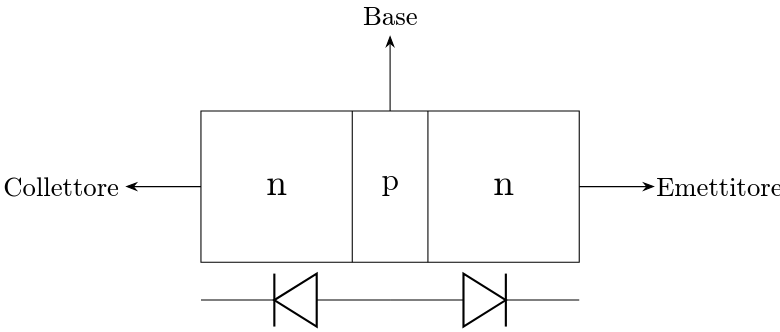
\includegraphics[width=\textwidth]{immagini/npn.png}
        \caption{Caption for image 1}
        \label{fig:image1}
    \end{subfigure}
    \hfill
    \begin{subfigure}[b]{0.45\textwidth}
        \centering
        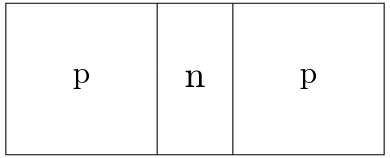
\includegraphics[width=0.75\textwidth]{immagini/pnp.png}
        \caption{Caption for image 2}
        \label{fig:image2}
    \end{subfigure}
    \caption{Overall caption for the figure}
    \label{fig:subfigures}
\end{figure}

Come è possibile notare dalle figure precedenti, da un punto di vista
circuitale i transistor BJT sono rappresentati utilizzando 3 terminali:
\(\to\) nel simbolo indica la giunzione (e ne è riportata solo una),
mentre le frecce indicano i versi delle tensioni (dove sono maggiori).
Parlando del transistor npn, per quanto riguarda le correnti abbiamo che
all'equilibrio \(I_B + I_C = I_E\), ed \(I_B, I_C\) sono entranti,
mentre \(I_E\) è uscente.

Per entrambe le tipologie di BJT, da un punto di vista costruttivo
valgono queste regole:

\begin{enumerate}
\def\labelenumi{\arabic{enumi}.}
\tightlist
\item
  La regione dell'emettitore è altamente drogata e ha il compito di
  emettere o iniettare portatori di corrente nella regione di base. Nei
  transistor npn, l'emettitore di tipo n immette elettroni liberi nella
  base, mentre nei transistor pnp, l'emettitore di tipo p introduce
  lacune nella base.
\item
  La base è sottile e leggermente drogata. La maggior parte dei
  portatori di corrente iniettati nella regione di base si muove verso
  il collettore senza fuoriuscire dal conduttore della base.
\item
  La regione del collettore è moderatamente drogata ed è la più grande
  all'interno del transistor. La sua funzione consiste nel raccogliere o
  attrarre i portatori di corrente iniettati nella regione di base.
\end{enumerate}

\section{Bipolar Junction Transistor: i
BJT}\label{bipolar-junction-transistor-i-bjt-1}

Il transistor BJT è stato il primo transistor ad essere prodotto su
larga scala, precedendo di una decade l'introduzione dei transistor ad
\textbf{effetto di campo}.

I BJT sono un dispositivo a semiconduttore a \textbf{tre} terminali,
realizzato tramite due giunzioni p-n.~Sono \textbf{bipolari} in quanto
il processo di conduzione coinvolge portatori di \emph{entrambe le
polarità}: quindi sia lacune che elettroni. \newline La realizzazione
fisica consiste nell'utilizzo di tre strati di materiale semiconduttore,
collegati ognuno ad un proprio terminale: abbiamo due strati esterni
composti con lo stesso materiale drogante (\textbf{collettore} ed
\textbf{emettitore}), ed un secondo strato posto tra gli altri due
all'interno del quale viene introdotto un materiale drogante opposto
(\textbf{base}). Così facendo otteniamo due giunzioni p-n: una
base-emettitore ed una base-collettore.

\begin{mybox}{\emph{Configurazione a diodi}}
In generale un transistor BJT è \textbf{quasi equivalente }a porre due diodi in antiserie\footnote{Antiserie indica, per bipoli polarizzati, una connessione in serie (quindi un solo punto di contatto), in cui le polarità dei terminali vengono accoppiate per segni uguali}. In realtà è più vicina una configurazione di due giunzioni p-n poste l'una di seguito all'altra e orientate in senso inverso (ognuna delle quali con la propria regione di svuotamento). Questo perché per \emph{far funzionare} il transistor BJT è necessaria la presenza di un'\emph{unica} regione di base, che svolge un ruolo cruciale nel controllo della corrente. Quando si affiancano due diodi, l'interazione tra le loro giunzioni non riproduce le caratteristiche di amplificazione e controllo della corrente tipiche di un BJT, in quanto l'introduzione di un metallo nel circuito non permette la corretta gestione delle correnti e delle tensioni necessarie per il funzionamento del transistor: non vi è il campo elettrico necessario a far passare gli elettroni da un diodo all'altro passando per il filo metallico.
\end{mybox}

È possibile realizzare la struttura in due diverse modalità:

\begin{itemize}
\tightlist
\item
  tipo \textbf{npn}
\item
  tipo \textbf{pnp}
\end{itemize}

I transistor npn sono usati più frequentemente. Inoltre le regole ed i
risultati ottenuti possono essere estesi ai transistor pnp modificando
opportunamente i versi di tensioni e correnti.

\subsection{Il BJT npn}\label{il-bjt-npn}

Un BJT npn è formato da due sezioni di tipo n (emettitore e collettore),
e da una di tipo p.~ Di fondamentale importanza per la fabbricazione di
un BJT è lo \emph{spessore della base}. Infatti deve essere il più
\textbf{sottile} possibile, senza fare un corto circuito tra le regioni
del collettore e dell emettitore.

In base alle polarizzazioni applicate alle giunzioni base-collettore e
base-emettitore, otteniamo 4 \textbf{regioni di funzionamento} del
transistor BJT:

\begin{table}[h]
\centering
\begin{tabular}{|c|c|c|}
\hline
\multicolumn{2}{|c|}{\textbf{Polarizzazione delle giunzioni}} & \multirow{2}{*}{\textbf{Regione di funzionamento}} \\ \cline{1-2}
\emph{B-E} & \emph{B-C} &  \\ \hline
Inversa & Inversa & Cutoff (Spento) \\ \hline
Diretta & Inversa & Attiva Diretta \\ \hline
Diretta & Diretta & Saturazione \\ \hline
Inversa & Diretta & Attiva Inversa \\ \hline
\end{tabular}
\caption{Regioni di funzionamento in base alla polarizzazione delle giunzioni}
\label{tab:reg-bjt}
\end{table}

\subsubsection{Regioni di funzionamento}\label{regioni-di-funzionamento}

\paragraph{Cutoff}\label{cutoff}

In questa regione il transistor è \emph{spento}. Entrambe le giunzioni
sono polarizzate inversamente: le rispettive tensioni sono ambedue
\textbf{sotto soglia}. In particolare \(V_{BE}<V_{\text{soglia}}\) e
\(V_{BC}<0\). \newline Dato che la giunzione BE non è polarizzata
\(\to i_B = 0\). Inoltre, dato che tutte le giunzioni sono polarizzate
inversamente, anche la corrente del collettore è \emph{nulla}.
\(\to i_C = 0\) \newline Nel grafico, la corrente non è esattamente
nulla dato che secondo la legge di \(I_D\) in una giunzione con
polarizzazione inversa la corrente vale \(I_O\).

\begin{quote}
In definitiva non vi è conduzione.
\end{quote}

\paragraph{Attiva diretta}\label{attiva-diretta}

In questa regione la giunzione BE è polarizzata \emph{direttamente},
mentre la giunzione BC è polarizzata inversamente. Significa che:

\begin{itemize}
\tightlist
\item
  \(V_{BE} > V_{\text{soglia}}\)
\item
  \(V_{BC} < 0\)
\end{itemize}

La corrente \(I_B >0\), e nonostante la tensione della giunzione BC sia
negativa, \(I_C= h_{fe}I_{b}\). \newline Dunque gli elettroni dovrebbero
ricombinarsi e ``richiudersi'' verso la base. Tuttavia, sapendo che la
base è ``corta'' gli elettroni raggiungono il collettore prima di
ricombinarsi, il quale li prende (forse meglio dire li accetta), in
quanto possiede un potenziale \emph{positivo}. È da notare che comunque
non tutti gli elettroni riescono ad attraversare tutto il transistor,
statisticamente alcuni si ricombinano con le lacune presenti nella
regione della base.

Il \footnote{È una funzione di.}\textbf{guadagno\footnote{In inglese è
  \textbf{gain}.} del transistor di corrente} è
\(h_{fe}=\frac{I_C}{I_B}\). Il transistor ha una funzione di
\emph{amplificatore} della corrente di base nel caso in cui \(h_{fe}\)
sia un valore alto: ciò lo rende \textbf{\emph{``attivo''}}

\begin{quote}
In questa regione funge da generatore di corrente controllato in
corrente.
\end{quote}

\paragraph{Saturazione}\label{saturazione}

In questa regione anche la giunzione BE è polarizzata direttamente:

\begin{itemize}
\tightlist
\item
  \(V_{BE}< V_{\text{soglia}}\)
\item
  \(V_{CE}<V_{CE -sat}\)
\end{itemize}

Se vale quest'ultima condizione (la tensione della giunzione BE è bassa)
allora anche BC è polarizzata direttamente. Per lo stesso motivo gli
elettroni non vengono ``raccolti'' dal collettore, tendendo a rimanere
nella base:

\begin{itemize}
\tightlist
\item
  \(I_{B}>0\)
\item
  \(I_C < h_{fe}\ I_{B}\)
\end{itemize}

\begin{quote}
È da notare come in questa configurazione/regione otteniamo una tensione
in uscita \textbf{costante} \(V_{CE - sat}\)
\end{quote}

\paragraph{Regione attiva inversa}\label{regione-attiva-inversa}

In questo caso \(V_{BE}<0\) e \(V_{BC} > V_{\text{soglia}}\). Quindi gli
elettroni si spostano nel collettore. In questo caso il *guadagno di
corrente è \(\leq 1\): \(\ I_{e} \simeq - I_{B}\).

\begin{quote}
Otteniamo un guadagno di corrente molto basso (tipicamente \(\leq 1\))
\end{quote}

\begin{figure}[H]
\centering
\begin{tikzpicture}
    \begin{axis}[
        axis lines=middle,
        xlabel={$V_{CE}$},
        ylabel={$I_C$},
        ymin=0, ymax=6, % adjust as needed
        xmin=0, xmax=6, % adjust as needed
        domain=0:5,
        samples=100,
        ytick=\empty,
        xtick=\empty,
        width=10cm, height=8cm,
        enlarge x limits=false,
        enlarge y limits=false,
        extra x ticks={1},
        extra x tick labels={$V_{CE(\text{sat})}$},
        extra y ticks={2.5},
        extra y tick labels={$I_{C(\text{sat})}$},
        axis line style={->}
    ]

    % Draw saturation region
    \addplot [fill=green, fill opacity=0.2, draw=none, domain=0:1] {2} \closedcycle;
    \node[rotate=90] at (axis cs:0.2,4) {Saturation Region};

    % Draw cutoff region
    \addplot[pattern=north east lines, pattern color=blue!50, draw=none, domain=1:5] {0} \closedcycle;
    \node at (axis cs:4,0.5) {Cutoff Region};
    \fill[white] (0, 0.01) -- (1, 2) -- (1, 0.01) -- cycle;

    % Draw curves for active region
    %\addplot[thick, black] {3*x/(x+0.5)};
    \addplot[thick, black] {2.5*x/(x+0.5)};
    \addplot[thick, black] {2*x/(x+0.5)};
    \addplot[thick, black] {1.5*x/(x+0.5)};
    \addplot[thick, black] {x/(x+0.5)};

    % Label the active region
    \node[rotate=45] at (axis cs:2.5,1.75) {Active Region};

    % Label currents for different base currents
    \node[right] at (axis cs:4.25,2.45) {$I_{B} = I_{B_3} + I_{B_2}$};
    \node[right] at (axis cs:4.25,2) {$I_{B} = I_{B_2} + I_{B_1}$};
    \node[right] at (axis cs:4.25,1.52) {$I_{B} = I_{B_1} > 0$};
    \node[right] at (axis cs:4.25,1.1) {$I_{B} = 0$};

\end{axis}
\end{tikzpicture}
\caption{Grafico BJT da completare}
\end{figure}

In questo grafico sono rappresentate delle curve che riportano gli
andamenti di \(I_C\) in funzione di \(V_{CE}\) con \(I_B\).

\subsection{Layout planare di un transistor
NPN}\label{layout-planare-di-un-transistor-npn}

\begin{figure}[H]
\centering
\resizebox{0.25\textwidth}{!}{%
\begin{circuitikz}
\tikzstyle{every node}=[font=\large]
\draw [thick, fill=blue!20](0,4.25) rectangle (5,0.25);
\draw [thick, fill=red!20]  (1,4.25) rectangle (4,2.25);
\draw [thick, fill=blue!20] (2,4.25) rectangle (3,3.25);
\draw [short] (0,1.25) -- (5,1.25);
\draw [short] (2.5,0.25) -- (2.5,-0.25);
\draw [short] (2.5,4.75) -- (2.5,4.25);
\draw [short] (3.5,4.75) -- (3.5,4.25);
\node [font=\large] at (2.5,0.75) {n+};
\node [font=\large] at (2.5,1.75) {n};
\node [font=\large] at (2.5,2.75) {p};
\node [font=\large] at (2.5,3.75) {n+};
\node [font=\normalsize] at (2.5,5) {Emettitore};
\node [font=\normalsize] at (3.75,5) {Base};
\node [font=\large] at (2.5,-0.5) {Collettore};
\end{circuitikz}
}%
\centering
\caption{Configurazione planare di un BJT npn}
\label{fig:my_label}
\end{figure}

Come mostra anche lo schema, da un punto di vista fisico il layout
planare di un transistor BJT npn \emph{non è simmetrico}: questo sia per
il drogaggio, sia per la realizzazione del dispositivo stesso.
L'emettitore è molto piccolo e molto drogato, mentre le regioni della
base e del collettore sono (viceversa) molto grandi e poco drogate.
\newline I contatti della base, dell'emettitore e del collettore sono
\emph{metallici} (se legati a zona n viene un diodo di silicio). Dato
che i materiali \(n^{+}\) sono molto drogati la regione di svuotamento è
molto piccola e gli elettroni la possono attraversare come se non ci
fosse.

\subsection{Il BJT pnp}\label{il-bjt-pnp}

È un dispositivo \emph{complementare} al pnp: valfolo le stesse
equazioni, ma tensioni e correnti sono \textbf{opposte} \newline Sia le
prestazioni che il guadagno sono \textbf{minori}, perché i portatori in
movimento sono le \emph{lacune}, più lente rispetto agli elettroni.

\subsection{Transistor ``speciali''}\label{transistor-speciali}

\subsubsection{Foto transistor}\label{foto-transistor}

Il phototransistor è caratterizzato da una corrente di base
\emph{``photo-generated''}\footnote{In questo caso la corrente di base è
  sostituita dall'intensità luminosa.}. Il resto dei parametri di lavoro
sono gli stessi un un normale BJT.

\[
I_C = k \cdot P_{L}
\]

dove \(P_L\) è la potente luminosa.\newline È importante che il
dispositivo si trovi in regione attiva: per questo sarà inserito un
resistore dal lato del collettore per evitare di andare in saturazione.

\begin{figure}[H]
\centering
\begin{circuitikz}[american]
\draw(1.0,-1.0) node[npn,photo,scale=0.59](Q1){};
\draw[short](Q1.C)to(1.0,-0.5);
\draw[short](Q1.E)to(1.0,-1.5);
\draw(2.0,-1.0) node[pnp,photo,scale=0.59](Q2){};
\draw[short](Q2.E)to(2.0,-0.5);
\draw[short](Q2.C)to(2.0,-1.5);
\end{circuitikz}
\caption{Un fototransistor npn ed uno pnp}
\end{figure}

\begin{figure}[H]
\centering
\resizebox{0.25\textwidth}{!}{%
\begin{circuitikz}
\tikzstyle{every node}=[font=\normalsize]
\draw (0,2) to[R] (0,0);
%\draw (0,0) to[npn, photo] (0,-2);
\draw(0.0, 0.0) node[npn,photo,scale=0.7](0,-3){};
%\draw[short={}](0.0,-2)to(-2.0,-3.0);
\node at (0,2) [circ] {};
\node [font=\normalsize] at (0.5,2) {$V_{CC}$};
\node [font=\normalsize] at (0.5,1) {$R$};
\node [font=\normalsize] at (2.25,0) {$V_{CE} = V_{CC} - R \cdot I > 0.2$};
\end{circuitikz}
}%

\label{fig:my_label}
\caption{Schema con fototransistor npn}
\end{figure}

\section{I transistor MOS}\label{i-transistor-mos}

I \textbf{MOSFET} (\emph{Metal Oxide Semiconductor Field Effect
Transistor}) sono una tipologia di transistor appartenente ai transistor
ad \textbf{effetto di campo}.

\begin{mybox2}{\emph{I transistor ad effetto di campo}}
I transistor ad effetto di campo sono caratterizzati dalla possibilità di controllare la
\textbf{conduttività elettrica del dispostitivo}, ovvero la quantità di corrente elettrica
che attraversa il dispositivo stesso, attraverso la formazione di un \emph{campo elettrico}
all'interno di esso. \newline
Possono essere realizzati in diverse modalità: 
\begin{enumerate}
\item JFET: ovvero Junction-Fet, realizzato con una giunzione p-n come elettrodo "rettificante";
\item MESFET: abbreviazione di Metal Semiconductor FET realizzato tramite una giunzione Schottky raddrizzante metallo-semiconduttore; 
\item MOSFET: il più comune.
\end{enumerate}
\end{mybox2}

Come per i transistor a giunzione, a seconda del drogaggio possiamo
ottenere due tipologie diverse di transistor MOS: i nmos e i pmos.

\subsection{N-Mos}\label{n-mos}

\begin{figure}[H]
\centering
\resizebox{0.7\textwidth}{!}{%
\begin{circuitikz}
\tikzstyle{every node}=[font=\LARGE]

\draw[thick, fill=red!20]   (0,7.25) rectangle (11,3.25); %rettangolo principale
\draw[thick, fill=yellow!20]   (4,8.25) rectangle (7,7.25); %ossido
\draw[thick, fill=blue!20]   (2,7.25) rectangle (4,6.25); %n+
\draw[thick, fill=red!60]   (4,9.25) rectangle (7,8.25); %metal gate
\draw[thick, fill=blue!20]   (7,7.25) rectangle  node {\LARGE n+} (9,6.25);%n+
\node [font=\Large] at (5.5,5.25) {P};
\node [font=\Large] at (3,6.75) {n+};
\node [font=\Large] at (5.5,8.75) {Metal gate};
\node [font=\Large] at (5.5,7.75) {Ossido di S};
\node [font=\Large] at (3,8.5) {Source};
\draw [short] (3,8.25) -- (3,7.25);
\draw [short] (8,8.25) -- (8,7.25);
\node [font=\Large] at (8,8.5) {Gate};
\draw [short] (5.5,10.25) -- (5.5,9.25);
\node [font=\Large] at (5.5,10.5) {Drain};
\draw (20,8.5) to[Tnmos, transistors/scale=1.02] (20,4.5);
\draw  (20.25,6.5) circle (1cm);
\draw [<->, >=Stealth] (12,5.75) -- (16,5.75);
\draw [->, >=Stealth] (21.75,5.25) .. controls (22.5,6.5) and (22.25,7.25) .. (21.75,7.75) ;
\draw [->, >=Stealth] (20,8.5) -- (20,7.5);
\draw [->, >=Stealth] (21,6.5) -- (20.5,6.5);
\draw [->, >=Stealth] (18.5,6.25) -- (19.25,6.25);
\draw [short] (19.25,6.25) -- (19.75,6.25);
\draw [short] (19.75,6.75) -- (19.75,6.25);
\draw [->, >=Stealth] (20,5.5) -- (20,4.75);
\draw [short] (20,4.5) -- (21,4.5);
\node [font=\Large] at (17.75,6.25) {Gate};
\node [font=\Large] at (20,8.75) {Drain $\sim$ C};
\node [font=\Large] at (22.25,4.5) {Source $\sim$ E};
\node [font=\Large] at (20.5,7.75) {$I_D$};
\node [font=\Large] at (20,4) {$I_S$};
\draw [->, >=Stealth] (19.5,4.75) .. controls (18.75,5) and (18.75,5.25) .. (18.25,6) ;
\draw [->, >=Stealth] (17.75,6) -- (17.75,5);
\node [font=\Large] at (17,4.5) {Terminale di controllo};
\end{circuitikz}
}%

\label{fig:my_label}
\caption{Transistor N-MOS}
\end{figure}

\printbibliography[heading=bibintoc]

\appendix

\chapter{Esercizi}\label{esercizi}

\begin{bluebox}{Le leggi di Kirchoff}
\begin{enumerate}
\item \emph{Legge di Kirchoff alle correnti}: la somma delle correnti in un nodo è pari a 0.
\item \emph{Legge di Kirchoff alle tensioni}: la somma delle tensioni lungo un percorso chiuso è pari a0.
\end{enumerate}
\end{bluebox}

\section{Esercizi capitolo 1}\label{esercizi-capitolo-1}

\begin{figure}[h]
\centering
\begin{circuitikz}[american]
\draw[V={}](2.0,-2.5)to(2.0,-5.5);
\draw[D={}](2.0,-2.5)to(6.5,-2.5);
\draw[R={}](6.5,-2.5)to(6.5,-5.5);
\draw[short={}](2.0,-5.5)to(6.5,-5.5);
\end{circuitikz}
\end{figure}

\chapter{Varie}\label{varie}

\section{Semiconduttori e bande}\label{semiconduttori-e-bande}

Gli elettroni in un solido allo stato fondamentale e a temperatura \(0\)
kelvin, in obbedienza alla loro natura fermionica e al principio di
Pauli che preclude ai fermioni il fatto di potersi trovare in due nello
stesso stato, riempiono gli stati elettronici loro consentiti partendo
dal livello energetico più basso via via su, fino a che tutti gli
elettroni del solido hanno trovato un'accomodazione. Si distribuiscono
cioè rispettando la distribuzione di Fermi-Dirac calcolata a temperatura
0 kelvin. Nei metalli, il livello energetico più alto occupato si
definisce livello di Fermi.

\begin{figure}
\centering
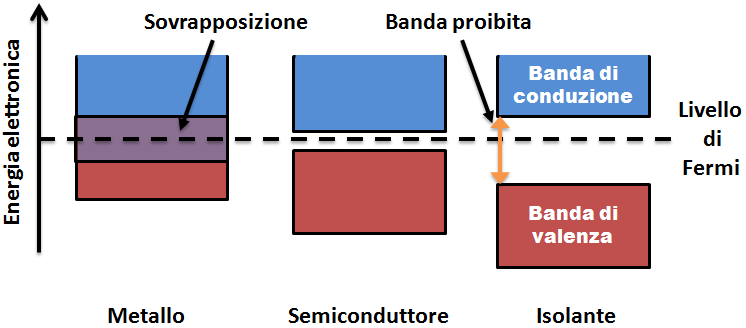
\includegraphics[width=0.5\linewidth,height=\textheight,keepaspectratio]{immagini/bande.png}
\caption{Schema semplificato della struttura elettronica a bande per
metalli, semiconduttori e isolanti.}
\end{figure}

A questo punto possono verificarsi diverse possibilità:

\begin{itemize}
\tightlist
\item
  Vi è una banda, o più di una fra le ultime riempite da elettroni, che
  è parzialmente riempita e restano degli stati vuoti. In tal caso si ha
  a che fare con un metallo, cioè un sistema in cui gli ultimi elettroni
  hanno la possibilità di spostarsi in livelli energetici molto vicini,
  infinitesimalmente più alti in energia, e dunque hanno la possibilità
  di una mobilità elevata che porta il sistema ad essere un buon
  conduttore di elettricità.
\item
  L'ultima banda è stata riempita completamente in modo tale che il
  prossimo stato elettronico consentito si trovi sulla banda successiva
  e fra questa banda e la banda completamente riempita c'è una banda
  proibita (\emph{band gap}) di energie. In tal caso il solido è un
  dielettrico.
\item
  Si parla infine di semiconduttore nel caso di un isolante in cui la
  banda proibita è talmente piccola che a temperatura ambiente c'è una
  certa probabilità che gli elettroni si trovino a saltare la banda
  proibita per agitazione termica, e dunque il sistema si trovi in una
  situazione prossima a quella di un metallo, con valori di
  conducibilità elettrica non nulli.
\end{itemize}

(N.B paragrafo proveniente da
\href{https://it.wikipedia.org/wiki/Struttura_elettronica_a_bande}{Wikipedia})

\begin{comment} 
TODO capire come funziona tavola periodica
## Tavola periodica

%%\pgfPT[show title=false, back color scheme=example,
%%  legend box={draw=blue!50,fill=blue!20},
%%  show extra legend,
%%  Z list={5,7,13,14,15,31,32,33,49,51}]
\end{comment}

\backmatter
\end{document}
